\documentclass[12pt]{article}
\usepackage[margin=3cm]{geometry}
\usepackage{blindtext}
\usepackage{chngcntr}
\counterwithin*{section}{part}
\usepackage{enumitem}
\usepackage{listings}
\usepackage{graphicx}
\usepackage{tikz}
\usepackage{subfig}
\usepackage{hyperref}
\usepackage{tcolorbox}
\usepackage{xcolor}
\lstset{language=C++,
    basicstyle=\ttfamily,
    keywordstyle=\color{blue},
    stringstyle=\color{red},
    commentstyle=\color{green},
    morecomment=[l][\color{magenta}]{\#}
}

\hypersetup{
    colorlinks=true,
    linkcolor=blue,
    citecolor=green,
    urlcolor=red
}
\usetikzlibrary{quotes, angles, decorations.markings, intersections}
\usetikzlibrary{calc,patterns,angles,quotes, 3d, intersections, positioning, shapes, automata, positioning}
\newcommand{\tbox}[1]{\noindent\fbox{\parbox{\textwidth}{#1}}}
\title{OS CS219 Notes}
\author{}
\date{\today}
\begin{document}
\maketitle
\setlength{\parskip}{6pt}
\setlength{\parindent}{0pt}

\noindent\tbox{
    \begin{center}
    \textbf{\Huge Lecture 1}
    \end{center}
}
\part{Introduction to Operating Systems}
\section{Introduction}
\noindent An \textbf{OS}(operating system) alias \textbf{Master Control Program} alias \textbf{System software} is software than enables the user to access the hardware resources of a computer 
in a controlled manner. It acts as a layer of abstraction allowing the user to not worry
about hardware level access and just provides access to a few methods needed by the user


\noindent The OS has several uses/functions in a computer
\begin{itemize}[topsep=0pt, partopsep=0pt, itemsep=0pt, parsep=0pt]
    \item Manages resources as a single \textbf{central entity} and hence efficiently
    \item \textbf{Virtualizes} physical resources to be utilized by multiple processes\footnote{process is defined later}
    \item \textbf{Isolates} and protects processes from one another by not allowing direct access to hardware 
    \item Provides a set of system calls for the user to access hardware resources
    \item Starts processes and allocates and manages memory required by said process during execution
\end{itemize}

\noindent Thus it is easy to see that the OS has several important functions to perform inorder to enable an abstraction of hardware from the users

\section{Process and Virtualization}

\noindent A process is just the sequence of execution of instructions by the CPU
. When we write and compile a program it gets converted into a sequence of instructions whose first \textit{instruction address} is fed to the PC and as we know 
the sequence of instructions for that program starts getting executed one by one. This is called a process. So when we run a program a \textit{process} is created.


\subsection{Context switching}
\label{section:context}
How do we tell the CPU to start a process. First obviously we need to feed the address of the first instruction of the process to the \textbf{Program Counter}. We also need to set 
the stack pointer and other registers with appropriate values. This is called \textbf{setting up the context} for a process. This job is done by the OS. After the context is set the OS takes a back seat and allows the CPU to do its work


\noindent However this has a few issues. Firstly, when the process requests for data from say the hard drive there is a gap where the CPU 
is on standby which is wasteful since other processes also require it. Secondly, we also want responsiveness from our system (ie) when
we have a process running we also may want to interact with other processes. 


Both of these issues are solved by \textbf{concurrent} execution. Basically we run a process for a while and when the CPU is on standby or after a 
particular interval of time we save the \textit{context} (ie) states of all registers including PC and start the other process by setting up its context this repeats
for a while and eventually the partially executed process's context is set and it is continued.
This is reffered to as \textbf{context switching} and is an important part of Virtualization\footnote{Read further to know what it is} of the CPU.
Note that a part of the OS (ie) \textit{OS scheduler} decides which program to run at what time

\subsection{Virtualization}
Virtualization refers to the creation of an illusion that each of the processes have full access hardware resources\footnote{It is useful to think of Virtualization as the OS lying to each process about it having full access to a resource}. This
enables the hardware to act much more powerfully than they are capable of. For example, as mentioned above context switching creates the illusion
of the presence of multiple cores each assigned to one process whereas in reality it is just one core.
Infact this is refered to as \textbf{Hyperthreading}. Apart from the CPU memory, addresses can be virtualized.

\section{Memory allocation and Isolation}
\label{section:mem_alloc}
\subsection{Memory}
As we learnt in CS230, memory for a process/program is allocated as a fixed number of bytes. The inital bytes
of this memory is the instructions and the global/static variables. Local variables aren't initialised in memory since
we do not know the number of times each function is called, instead we have a dynamically growing stack whose starting address is
stored in the special \textit{stack pointer register}. This stack grows and shrinks as necessary functions are called and they return values.
\footnote{The structure used here is a stack since functions are inherently \textit{LIFO} functions called last return first}.


Apart from this we have a heap which can be accessed by user to store dynamically increasing data structures. We can request the
OS to allocate certain number of bytes and return a pointer to said bytes


Here again however the OS plays tricks on the processes. Since it is impractical for the OS to allocate to 
allocate memory for the process continguosly it allocates them in chunks but returns a \textbf{virtual address} (Recall Virtualization) to the program. This "virtual address" is the
address returned when the user requests the OS for an address of the data stored. Here again the OS lies to the process creating the illusion that it has access to continguos memory starting
from some location

\noindent\tbox{
    \begin{center}
    \textbf{\Huge Lecture 2}
    \end{center}
}
\subsection{Isolation}
    \label{section:Isolation}
    Now we understand that the OS allows multiple processes to run at the same time and share resources
    But this raises a huge issue since processes are supposed to be independent and processes being to affect other 
    processes would cause problems. The OS takes care of this too by maintaing strict control over access to hardware

    The OS is the only entity with access to hardware and process can make specific requests to the OS to use hardware
    via \textit{system calls}\footnote{syscalls can't be accessed directly usually. They are in a language's standard library}. Infact there are two types of instructions and processer modes corresponding to them

    \begin{itemize}[topsep=0pt, partopsep=0pt, itemsep=0pt, parsep=0pt]
        \item \textbf{Privileged instructions} - special instructions that can interact with hardware. Generated by syscalls,device drivers
        CPU is in \textbf{kernel} mode while executing them 
        \item \textbf{Unprivileged instructions} - simple instructions that do not need access to hardware. Given by user processes. CPU is in \textbf{user} mode while running them
    \end{itemize}

    The CPU is always in user mode except the following cases.
    \begin{itemize}[topsep=0pt, partopsep=0pt, itemsep=0pt, parsep=0pt]
        \item A syscall is made
        \item Interrupt occurs
        \item Error needs to be handled 
        \item Context switching needs to happen for say concurrent running
    \end{itemize}
    
    Note that when a syscall is made the OS code pertaining to it is executed and then control is return back to user code
    \\\textbf{Interrupt:} In addition to running programs a CPU has to handle external inputs from devices like a mouse click.
    This is called an Interrupt. During an interrupt control is given to the OS(Kernel mode of CPU) which deals with the interrupt and returns
    control to the user process \footnote{This means saving context, handling the interrupt and setting context of the past status}


    \noindent\textbf{Device Driver:} I/O is managed by the device controller(Hardware) and device driver\\(software)\footnote{This is part of the OS}.
    The driver initializes IO devices and it starts IO operations like reading from the disk. It also handles the above mentioned interrupts


    \section{Process abstraction and attributes}

    As we have discussed above about a process it is a sequence of instructions running in the cpu.
    Also as discussed in section \ref{section:context} a process can run for a while, then be blocked and run again.
    Hence a process switches from one \textit{state} to another during its execution. We can note that this process state changes only when the kernel goes to user mode.\footnote{Since the change is done by the kernel's OS scheduler}

    \begin{figure}[h]
        \centering
        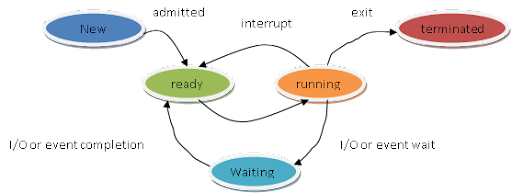
\includegraphics[width = 10cm]{process-state.png}
        \caption{Figure to show process state switching}
        \label{process-state}
    \end{figure}
    {\large A process is defined by several \textit{attributes} that define it:}
    \begin{itemize}[topsep=0pt, partopsep=0pt, itemsep=0pt, parsep=0pt]
        \item \textbf{PID}: Unique process identifier given to each process
        \item \textbf{PPID}: PID of a parent process\footnote{Parent discussed later}
        \item \textbf{Context}: Context is saved when switching happens. We have discussed what the context of a process refer \ref{section:context}
        \item \textbf{File descriptors}: A record of all the files open by a process is stored in form of pointers in 
        an array. Elements at index 0,1,2 refer to std input, std output and error files. As we open more files for
        a process a pointer to it is created and added to the end of the array. This poiner is what is returned as a 
        \textit{file descriptor} for the user to perform read or write operations.
        \item \textbf{State}: A process can be in 3 states
        \begin{enumerate}[topsep=0pt, partopsep=0pt, itemsep=0pt, parsep=0pt]
            \item \textbf{Running}: The CPU is currently executing instructions of the process
            \item \textbf{Blocked/suspended}: The process cannot run for a while. Maybe it requested data from drive and is waiting for its arrival
            \item \textbf{Ready/runnable}: Process can be run and is waiting for \textit{OS scheduler} to give it a CPU/core to use
        \end{enumerate}
        \item \textbf{Memory}: Each process uses/is allocated a fixed amount of memory by the OS and its locations are stored
        \item \textbf{Page Table}: The OS lies to the process about memory addresses(Virtual address \footnote{refer Section \ref{section:mem_alloc}}). The real address mapping to the corresponding
        virtual address is stored in the page table. The page table can be used to get the real address corresponding to each virtual address
        \item \textbf{Kernel Stack}: The context of a CPU is saved in this kernel stack when context switches occur. This stack is stored in a seperate memory and it isn't accesible by user code
        The OS uses this stack since it doesn't trust the user stack. Each process has its own kernel stack
    \end{itemize}


    \subsection{Process Control Block}
    All the above mentioned attributes of a process along with more necessary information
    is stored in a data structure called the process control block(PCB)\footnote{Stores the details about one process}


    It is called by different names in different OSes:
    \begin{itemize}[topsep=0pt, partopsep=0pt, itemsep=0pt, parsep=0pt]
        \item \textit{struct\_proc} in xv6
        \item \textit{task\_struct} in linux
    \end{itemize}


    The above mentioned attributes of various processes are stored in the PCB 
    in form of the \textbf{ptable} or process table which is a data structure storing all the 
    \textit{proc structs} each of which has all the data corresponding to each process

    In \textbf{xv6} the ptable is just an fixed size array since it is a simple system. However in real
    world kernels it is a dynamically expanding data structure. 

    
    The \textbf{OS scheduler} iterates over the ptable picks a \textit{ready} process and assigns it a processor to run it.
    A process which needs to be put to sleep (Eg. IO from disk) will be put to sleep and another is picked from processor
 
    \section{Booting}
    We need some system to load up our OS into the CPU during start of the system.
    The \textbf{BIOS}(Basic input output system) is present in the non-volatile memory of our system which locates boot loader 
    in the boot disk. It is a simple program whose job is to locate and load the OS. It is present in the first sector of the boot disk
    It sets up context for the kernel and gives control to kernel


    \textbf{BootLoader} must fit in 512 bytes of the Boot disk to be easily located which isn't sufficient to load up current complicated systems.
    So the 512 bytes(simple bootloader) load up a more complex BootLoader which loads OS onto the CPU 
\newpage
\noindent\tbox{
    \begin{center}
    \textbf{\Huge Lecture 3}
    \end{center}
}

\part{Process Management}
\section{API:Application Programming Interface}
\textit{System calls} provide an interface to the OS called the Application Programming Interface (ie) the set of syscalls given
to the user constitute the \textbf{API},

Two types of syscalls are:
\begin{itemize}[topsep=0pt, partopsep=0pt, itemsep=0pt, parsep=0pt]
    \item \textbf{Blocking:} Syscalls that block the process that called it\footnote{Like when you wanna read from disk which takes time} and the OS comes back to the user process after a while
    \item \textbf{Non Blocking:} Syscalls that are called with the user instructions which acts along with user process without blocking the calling process\footnote{The process which calls the syscall} since they return immediately (eg. getpid())
\end{itemize}


If every OS has different syscalls \textit{portability}\footnote{ability to run same code on multiple machines} is an issue. For this purpose all the OS providers decide on an universal set of syscalls
\footnote{The implementation of said syscall may differ} to provide called the \textbf{POSIX} API. Interestingly, since the instructions for syscalls maybe different this is why we may have to recompile to run code on another OS

Hence the hierarchy of a syscall is somewhat like:
\begin{center}
    User code $\rightarrow$ Standard library functions $\rightarrow$ Syscall in the function $\rightarrow$ Syscall in assembly instruction $\rightarrow$ OS
\end{center}

In xv6 we are directly given syscalls in the standard library in a user friendly function call. Usually we are given syscalls at the assembly code level
since we usually need to change the privilege of CPU\footnote{Done using INT in assembly}. Hence we need to understand that syscall is \textbf{NOT} a regular function call.\footnote{Lottt more detail on this further}

\subsection{Fork}
Each process is created by another process. Such a process emerging from another is called the \textit{child} of the \textit{parent} process.
The syscall used to create such a process is called \textit{fork}. \texttt{Init} is the initial process from which all other processes are \textit{forked}.

When you call fork:
\begin{itemize}[topsep=0pt, partopsep=0pt, itemsep=0pt, parsep=0pt]
    \item New child process is created with new \textbf{PID}
    \item Memory image\footnote{the heap,stack,instructions,data is the memory image of a process} of the parent is given to the child
    \item They run copies of same code
\end{itemize}
Note that while the child may share the virtual memory with parent. It is in a different physical memory location


What is the point of running the same process as a child again? There is none. They aren't the same process due to one key difference.
The \texttt{fork()} returns 0 in the child process and returns the PID of child to the parent. Hence we can make the parent and child run different code
using the different value returned by the \texttt{fork()} function. Note that \texttt{fork()} returns -1 when forking fails. This process seems to be generating different process running some redundant code.
This is not the way to create process to perform very different functions as compared to parent.
We will see another way to create processes for that case
later. Interestingly as of yet the parent also needn't run before the child since they are independent processes

We can also have nested forks as in multiple forks() in a program. This will make a parent and the child each of which will also call another fork and so on.


\textbf{xv6 fork() code:}
\begin{itemize}[topsep=0pt, partopsep=0pt, itemsep=0pt, parsep=0pt]
    \item Allocates memory for new process and gets PID
    \item "np" a pointer to struct proc of child is created
    \item "currproc" points to struct proc of parent
    \item Copies info from currproc to np
    \item Child is made runnable and put on ptable and PID is returned in parent and 0 in child
\end{itemize}

\newpage
\noindent\tbox{
    \begin{center}
    \textbf{\Huge Lecture 4}
    \end{center}
}
\subsection{Exit and wait}
When a process is done it calls exit() to terminate. Exit is called at the end of main() automatically.
Exit doesn't clean up the memory of a process and the process is in a dead \textbf{Zombie} state.

Parent process of a child calls wait() syscall which cleans up the memory of a zombie child and returns the PID of said zombie process(or -1 if no child). If wait() is called in the
parent before child is a zombie the parent is suspended and waits till the child is 
running. You can also call waitpid() which reaps only a process with a particular pid whereas in normal 
wait() some arbitrary process out of all zombied ones processes are reaped. Note that one wait() reaps only one child. So we need a wait() for every fork().


What if parent dies without calling wait(). Then the child continues to run as an orphan process. In this case \texttt{init.} 
adopts the orphan process and becomes its parent and eventually reaps\footnote{calls wait() and erases the memory of the zombie} it. This is done when the parent calls exit which makes all the parent
pointers of its children point to \texttt{init.}. Note that \texttt{init.} comes into play iff the parent dies, not when it is alive in anycase. So \texttt{init.} keeps
checking if there is an orphan to adopt and eventually reap. If parent is alive but doesn't call wait then system memory fills with zombies\footnote{ahhhhhhh apocalypse}


\subsection{Exec}
As we saw the fork() method seems complicated with if-else blocks for parents and children and there seems to be redundant code. We create
child to do similar work as parents lots of times. If this is not the case (ie) parent, child are doing different things(and we don't want the parent around) we can use \texttt{exec}.
exec() is used to get a new memory image(using that of the old process) which is used to run an executable which it takes as an argument. It is not similar to fork() since it doesn't create a new memory image
it just replaces the parent's memory image and it copies the executable's memory image to run the executable. The ptable is also updated with the new details of the process\footnote{but the PID,PPID is the same}


So whatever code is given after exec is never run by the child since it overwrites the parents memory image with the executable given as a argument. However if 
exec fails then the parent's image copy only is present in the new process and thus all the code after exec in the parent is run by the child once it gets access to the CPU. 


\noindent\tbox{
    \begin{center}
    \textbf{\Huge Lecture 5}
    \end{center}
}
\section{Shell}
Shell is the process which handles accepting and executing terminal commands
\begin{lstlisting}[language=C++,caption = Shell code]
    while(1){
        input(commands);
        int ret =  fork();

        if(ret == 0){
            exec(command);
        }
        else{
            wait();
        }
    }  
\end{lstlisting}
The basic working of the shell goes like this:
\begin{itemize}[topsep=0pt, partopsep=0pt, itemsep=0pt, parsep=0pt]
    \item Shell forks a child which calls exec to run commands
    \item Why doesn't the shell call exec() itself. This is since we want the shell program to keep running and not get replaced
    \item Some commands have code written in the OS itself like \texttt{cd}, since they need to maintain the pwd\footnote{present working dictionary} while others
    have executables called by exec() like \texttt{ls}.
    \item User commands run in \textit{foreground} (ie) can't accept next command till previous one is done
    \item \textit{Background execution} is when we give a command followed by \& the shell runs command but doesn't wait for it to finish.
    So reaping is taken care later by the shell using a method where wait is invoked without blocking parent.
    \item We can also run multiple commands in \textit{foreground} sequentially(one after another) using \&\& or parallely using $||$ 
\end{itemize}


Some things taken care by the shell:\\\\
\textbf{I/O redirection:}
Every process has some IO channels or "files" open which can be accessed by file descriptors\footnote{STDIN.STDOUT,STDERR}.
Parent shell can manipulate these files descriptors of child before exec() to do stuff like I/O redirection (ie) by changing the STDOUT file to out desired file or STDIN to desired file.
Basically the process still thinks its getting from STDIN or outputting to STDOUT but we change the file descriptors to point to files we want, essentially tricking the process to output/input to/from the desired file


\textbf{Pipes:}
Pipes are when the output of one command is given as input to another command.
Shell creates a temporary buffer in OS called well a "pipe" and the STDIN-file descriptor of the other command process is made to point to the 
"pipe". Basically pipe is redirected as input to the next commands.


\textbf{Signals:}
Signal is a way to send notifications to process.(eg. kill -9 PID\footnote{SIGKILL}). There are some standard signals available to each OS. SIGINT, SIGCHLD, SIGTERM, SIGKILL\footnote{Interrupt,signal to parent when child terminates,terminate,kill respectively}\\....etc.
Note that the kill command can send all signals and which signal it sends is determined by id in "kill -id pid" which conveys the signal. The OS can also
generate signals on its own and not from processes(eg. CTRL + C sends SIGINT).


When we send a signal it is sent to all the processes in that process group. A process group is an organisation where sets of processes
are treated as group. By default a process belongs to its parent's process group. CTRL + C sends SIGINT to all processes of the \textit{foreground} process group
. The syscall \texttt{setpgid()} can be used to change the process group of a process.


Signals to a process are queued and delivered to the OS which handles them. It knows to ignore certain signals and to 
make some processes stop for certain others. User processes can also define their own signal handlers using the signal syscalls to overwrite default behaviour.
 The process jumps to the process's signal handler and back to the process if it exists after signal is taken care of.
However note that some signals like SIGKILL can't be overriden by a process's signal handler since the OS needs to maintain some power over process incase they go rogue.
\\
\newpage
\noindent\tbox{
    \begin{center}
    \textbf{\Huge Lecture 6}
    \end{center}
}

\section{Trap handling}
\label{section:trap}
As we saw before the CPU can execute instructions in User mode or Kernel mode with differing level of privileges\footnote{Refer \ref{section:Isolation}}.
The process of going to Kernel mode is called a "Trap" the CPU \textit{traps} into the OS code via the running process\footnote{read further to find out what a trap is}.
The OS isn't a seperate processes it just runs in the same process which called it (by trapping the OS) just in the Kernel mode of the CPU.

Note: Random doubt, How are interrupts and signals different. Interrupt is a message from a \textit{device} to the system which is handled by OS.
Signal is a message sent from one process or another. When we give CTRL + C that is an \textit{interrupt} from the keyboard which the OS handles to create a \textit{SIGINT} signal to the running process

Why is a sycall() even different from a function call??
To understand lets see what happens when a function call is made
\begin{itemize}[topsep=0pt, partopsep=0pt, itemsep=0pt, parsep=0pt]
    \item Allocation of memory on stack for function arguments, local variables. Note that this doesn't happen during function definition.
    \item Push return address and PC jumps to function code
    \item Save register context of the calling process
    \item Execute function code and once done pop return address and pop register context
\end{itemize}

In a syscall some similar things are done
\begin{itemize}[topsep=0pt, partopsep=0pt, itemsep=0pt, parsep=0pt]
    \item Push return address and PC jumps to function code(How does the user know where OS code is?)
    \item Save register context for the calling process
    \item Execute function code and once done pop return address and pop register context
\end{itemize}

But the important difference is \textit{where} the memory for the syscall() variables are allocated and what information is exposed to user.
We can't expose the PC locations for various syscalls since they can be misused and abused by the User. It also completely takes away control from the OS and leaves the system vulnerable to attacks.
Also the OS is \textit{paranoid} in the sense that it is designed to not trust the user. Since the User has access to the user stack the OS doesn't use that stack
for allocating variables for its syscall(). It rather has its own secure \textbf{kernel stack} which is not accessible to the user.

\subsection{Kernel stack and IDT}
The kernel stack is used for running all the OS code. There is a part of the PCB given to these secure OS processes which aren't accessible to the user.
The context for a process calling a syscall is pushed onto the Kernel stack and is popped when the syscall is done.


Again how does a process know which PC to jump for a syscall(). We have the \textbf{Interrupt descriptor Table} for this purpose.
It is a special data structure which has the mapping to the PC at which each syscall()'s code is present. This PC is indexed by n which is the 
argument passed to the \textit{trap} instruction. Accessing this table can only be done by privileged instructions.


When the user wants to make a system call we can't do it with OS code directly since it involves changing permission to Kernel mode which the OS code needs anyway to run\footnote{problem of which rat will bell the cat}. We obviously can't make the user
code do it due to \textit{lack of trust}. The only trust worthy entity which is capable of changing permission to run OS code is the hardware. The hardware creates an interrupt which calls a special "trap instruction" or (INT n) at the assembly code level with an argument which indicates the 
type of trap(to indicate which syscall,interrupt,error is calling it). After this the CPU is finally capable of running OS code and thus OS can perform whatever the trap was called for.


The \textbf{IDT} is setup during Bootup of a system to give the PC's of syscall() depending on which task is to be done.
This PC is used by the interrupt instruction to jump to a syscall()'s PC thus maintaining security. Thus, note that the \textbf{IDT} is a very important data structure and 
an ability to compromise it can give access to the entire system since we can locate where all the OS's code and virtual memory is and thus gain access to the entire system 


How does trap make the privilege to \textit{Kernel mode}? What all does it do?
\begin{itemize}[topsep=0pt, partopsep=0pt, itemsep=0pt, parsep=0pt]
    \item CPU privilege is increased
    \item CPU shifts it's stack pointer to the kernel stack
    \item The user context for the calling process is saved(for a syscall)
    \item The PC (can be obtained from interrupt table) is changed 
\end{itemize}


Now we are in a position to start running the OS code. After the OS code is done handling the syscall/interrupt, it calls a return-from-trap
instruction(Trapret and iret).
\begin{itemize}[topsep=0pt, partopsep=0pt, itemsep=0pt, parsep=0pt]
    \item CPU privilege is decreased
    \item CPU shifts it's stack pointer to the User stack
    \item The user context for the calling process is copied to CPU
\end{itemize}
User is unaware that it was even suspended and continues as if nothing happened.

\textbf{IDT Lookup: }The IDT is basically an array whose starting index is stored in a CPU register and the interrupt number 'n' given in INT n is the index of the PC we need.
\noindent\tbox{
    \begin{center}
    \textbf{\Huge Lecture 7}
    \end{center}
}

\subsection{Trap Frame in xv6 and trap handling}
\begin{itemize}[topsep=0pt, partopsep=0pt, itemsep=0pt, parsep=0pt]
    \item A data structure called the Trap frame is pushed onto the kernel stack when a trap is encountered and then it is popped by return-from-trap
    \item It contains various register values to be saved and not get lost during trap handling (pushed by OS).
    \item The "int n" pushes a few registers w(PC,SP etc.) and jumps to kernel to handle the trap and the rest of the registers are pushed by kernel code after which trap handling is done
    \item \textbf{EIP,ESP} has values that get modified as soon as the "int" instruction is completed. So we need to save them with the int n instruction itself and cannot wait for OS code.
    \item IDT entries for all interrupts set the EIP to point to the kernel trap handler "\texttt{Alltrap}" which is common for all traps into the OS regardless of the reason for why the trap was called
    \item \texttt{Alltrap's} assembly code pushes remaining registers to complete trapframe on Kernel Stack
   \\ Note: Why do we have to save registers doesn't the \texttt{int} instructions do it for us? The hardware only saves the bare minimum and absolutely required values like \textbf{EIP,ESP}.
   It is upto the OS to save the remaining registers (depending on if it needs to) inorder to restore them after trap handling
   \item Thus after \texttt{Alltrap} is executed our sturct Trap frame has all its values set appropriately
    \item Note that after the \texttt{Alltrap} is completed the ESP points to the top of the trap frame
    \item After this we invoke the \texttt{trap()} function in C which actually handles the specific reason the trap was called for\footnote{It knows the reason from the value of the eax register which it passesn as an argument, int n}
\end{itemize}

So we can see that \texttt{\texttt{Alltrap}} is written in assembly to do the bare minimum that \textbf{must} be done in assembly like pushing registers to Kernel stack. After this we go to a high level
language like C enabling us to code the logic in the more compliacted part of actually handling the trap much easier. 
After the trap handling is done the assembly code \texttt{trapret}'s instructions are executed. This pops the trapframe from the kernel stack (things pushed in the \texttt{Alltrap}s). It calls the \texttt{iret} instruction which is the opposite of int. It pops values which int pushed to kernel stack after which it changes privilege level back to user mode. After this the process which trapped the OS continues running. In xv6 if it was a syscall that called the trap after all the trap handling is completed the OS puts the return value for the 
syscall in the \texttt{eax} register.


So in conclusion the int instruction and \texttt{Alltrap}s work together to save values when a trap is performed. C code(trap handler) takes care of the actual trap. Trapret pops the register context and \texttt{iret} returns from trap and control goes back to user


Depending on the value at n we know if the int was called for a syscall or an interrupt and can handle it appropriately. How do we know when a device interrupt occurs?
If a particular pin connected to the device has a high value then an 
\texttt{int n} in passed to the CPU with an appropriate "n" value and thus the CPU can handle the device interrupt


\subsection{Timer interrupt}
\label{section:Timer}
We thus understand how a trap can give control to the OS. But it maybe that intentionally or accidentaly that a program never does a trap. So the OS would never get the control
of the CPU. What if such a process goes into an infinite loop? How will the OS stop it? Alternately if we want to do a context switch how will the OS get control? One option is to just assume the process
is not malicious and it is smartly written to trap into the OS at regular intervals. However the better option is to interrupt every process after a particular amount of time has passes and then 
trap into the OS to handle this interrupt and check if everything is okay or do a context switch if required. This interrupt is appropriately called an \textbf{Timer interrupt}. The Timer interrupt is a special hardware interrupt and is given to kernel periodically.

\noindent\tbox{
    \begin{center}
    \textbf{\Huge Lecture 8}
    \end{center}
}
\section{OS scheduler}

OS maintains a list of all active processes in a data structure. Processes are added in during \texttt{fork()} and it is removed during \texttt{wait()}.
The \textbf{OS scheduler} is a piece of ccode that runs over this dynamically growing data structure and picks a process to run.
Basic Job of the scheduler:
\begin{itemize}[topsep=0pt, partopsep=0pt, itemsep=0pt, parsep=0pt]
    \item It saves the context of the currently running process in its PCB
    \item Loops over all the ready processes and picks a process to run(according to its policy)
    \item Restore context of the new process from PCB and make it run
    \item Continue as long as system is active
\end{itemize}

Why do we want to do context switch?
Sometimes when OS is in kernel mode it can't go back to the process which it trapped into. For example, when the process has terminated or when it has made a blocking system call.
Another reason could be that the OS may not want to return to the same process due to the necessity to give fair oppurtunity for all process to run. This is done through \textit{time sharing} for which context switching is necessary.

The OS scheduler needs to decide on a policy (\textit{scheduling policy}) for selecting a process to run and needs to have a mechanism to switch to that process. The scheduler can be non pre-emptive where it switches contexts only
 when a running process does a blocking syscall or gets terminated ie when it willingly gives up control. A pre-emptive scheduler will perform a switch even if a process is ready to run. It does this via timer interrupt\footnote{Refer \ref{section:Timer}}



\subsection{Mechanism of a context switch}
 How does a context switch happen? Assume we want to switch from process A to process B. Process A is trapped into OS\footnote{Refer \ref{section:trap}}. Kernel stack has register context of user process A in the trap frame.
 After running some kernel code assume process A can't be run anymore (Say it asked to read from disk which takes time). Now we want to switch to B. 

 We now save the \textit{Kernel context} (ie) PC of OS where we stopped, kernel stack pointer, some registers etc.. . Now be careful and observe that there are \textbf{two different} contexts the \textit{user context} and the \textit{kernel context} of a process.
 The user context is saved on the kernel stack by a trap into the OS from that process. The kernel context is saved on the kernel stack during a context switch.
 After saving both contexts we then switch the value of the stack pointer to the kernel stack of B\footnote{The switching of this stack is the exact moment of the context switch} from the kernel stack of A\footnote{each process has its own Kernel PC}. 

 What does kernel stack of B have? It trapped into OS at somepoint or was context switched out. So its kernel stack has a trap frame, kernel context etc... . We now restore the kernel context
 of B and resumes execution in kernel mode of process B at the point(ie at the PC where context switch happened) the CPU was given up by it\footnote{This is why we store the kernel PC when we context switchd out of A}. Now user process B can run as normal after it returns out of trap.
 Thus we have completed a context switch. 
 
 
 An important point to note is that \textit{context swtiching }can only happen in kernel mode. So when we switch context the \texttt{EIP} is an OS code PC. When we switch into another process we switch into the OS code PC 
 address which we were about to execute the last time a context switch happened with the process we are switching into. That is the PC of the last OS code B was executing before the last time it got switched out.\footnote{This point is quite confusing. A helpful hint is to try to visualise what happened that last time a context switch happened with B which stopped it from running}

 What if B is a new process that has never been run before? Since it as never context swtiched before will it have its \textit{kernel context} saved? We can create a new process only by calling
 \texttt{fork()} and fork doesn't create an empty kernel stack. It gives some dummy value to the stack which solves this issue. We will look at this issue in detail later

 \subsection{OS scheduler in xv6}
 In xv6 every CPU has a scheduler thread ie a special process for the scheduler code. Also note that xv6 is a pre-emptive scheduler with timer interrupts. It runs over the list of processes and then switches to one of the runnable ones. 


 The scheduler process runs and then it context switches to another process. When the current process wants to switch to another process it swtiches to the scheduler and then to another process. 
 Direct context switching doesn't happen. The scheduler is always a middle man.

{\texttt{sched():}}  xv6 has a function \texttt{swtch()} that actually performs the context switch. The \texttt{sched()} functions makes the process context switch to the scheduler. It can't be called in user mode. It
is a OS function to be run in kernel mode. The calling process is switched out and the scheduler context is switched in. The scheduler then finds out 
some other process to run and then \texttt{swtch()} context switches from scheduler to that process. 

When does a process call \texttt{sched()}:
\begin{itemize}[topsep=0pt, partopsep=0pt, itemsep=0pt, parsep=0pt]
    \item \textbf{Yield:} Timer interrupt occurs, process has run enough and gives up CPU
    \item \textbf{Sleep:} Process performed blocking action like I/O from disk
    \item \textbf{Exit:} Process called exit, sets itself as a zombie and gives up CPU
\end{itemize}

In both the scheduler,\texttt{sched()} function the function \texttt{swtch()} switches between two contexts.

\textbf{Context structure:} It is the set of registered stored/restored during a context switch from one process to another. As disucssed before it is pushed into the kernel stack during a context switch.
The pointer to this structure is stored in the \texttt{struct proc} of the xv6 system as a field called "context"(p$\rightarrow$context). This could be thought of as similar to the \textit{kernel context}.


Note that the trap frame is a different structure which also has its own pointer in \texttt{struct proc} even though it is also stored on the kernel stack. It is saved during a trap into the OS whereas \textbf{context structure}
is stored only during a context switch. An example is a timer interrupt, when the process traps into the OS itself the \textbf{trap frame} is saved whereas the \textbf{context structure} is only saved during a 
context switch to a different process

\noindent\tbox{
    \begin{center}
    \textbf{\Huge Lecture 9}
    \end{center}
}
\\
\subsection*{Reference: Caller and callee saved conventions}
\textbf{Caller and callee saved registers:} Registers can get used and the values they had before maybe lost
when they are used to execute code from a function call. Some registers are saved on stack by caller before involving the function(caller\footnote{the code which made the function call} saved)
and then these can be modified by the function (callee\footnote{the actual function call code}) freely without the callee have to worry about saving them.

Some registers saved by callee function and restored after function ends (callee saved). Caller code
can expect them to have same value on return and doesn't have to save them on its own. 

An example is that the \textbf{return value} is put by callee in \texttt{eax} thus the previous value in it is lost. Thus the caller must be save it. The 
work of saving registers to make sure they aren't lost in the function execution.
These things are taken care of by the C compiler so the programmer doesn't need to take care of them. 


There is a very specific convention on what registers are pushed and popped in which order when a function call is made.
It is as follows:
\begin{itemize}[topsep=0pt, partopsep=0pt, itemsep=0pt, parsep=0pt]
    \item Push the caller save registers(\texttt{eax,ecx,edx})
    \item Push arguments in reverse order
    \item Return address (old \texttt{EIP}) is put on stack by call instruction(callee saved)
    \item Push old ebp on Stack
    \item Set \texttt{ebp} to current top of stack (base of new "stack frame\footnote{the portion of the stack given for the function execution}")
    \item Push local variables and callee save registers(\texttt{ebx,esi,edi})
    \item Execute the function code
    \item Pop stack frame (of the function call) and restore old ebp 
    \item Return address popped and \texttt{eip\footnote{instruction pointer}} restored by the \texttt{ret} instruction to jump back to the caller instruction

\end{itemize}

Thus it is easy to see that in a way the callee saved registers are those absolutely essential for the function call to be returned properly like \texttt{ebx,esi} and the rest of the
registers are saved according to the needs of the caller.
\\\textbf{Stack pointers}: \texttt{ebp} stores base of stack frame and \texttt{esp}(changes with growth of stack) stores the current top. Thus we can access the full of the stack this way.
We can also very easily access arguments since they are on the base of the stack

\subsection{\texttt{swtch()} in xv6}
It first saves the registers in the context structure onto the kernel stack of the old process.
It now switches ESP(stack pointer) to context structure of the new process. Pops the registers from the new processes context sturcture(the moment context switch is happening).
CPU now has the context of the new process. This entire process is coded out in assembly language since we have to push and pop
registers from the stack which cannot be done in c.



\subsubsection{Parameters of \texttt{swtch()}}
Both the CPU thread and the \textit{struct proc} stores the pointer variable to the
context structure. \texttt{swtch()} has two arguments(two pointers a context** and a context* pointer). It is the pointer to the old context (ie) current 
process's context pointer (Note that this is the pointer to the context pointer) and the context pointer of the process we want to switch into. 


We take the pointer to the context pointer(\&(p$\rightarrow$context)) of the process we are switching from and not the context itself(p$\rightarrow$context)
for an important reason. We want to update the context to its latest status. What we mean is that when we context switch out of a process it already has the last context which
it had when it was switched out previously. We want to update this context to the current value since when we come back to the process in the future we want to start executing it from
this point which we are leaving it at.

We however needn't modify anything about the context of the process we are switching into but rather just wants its value. Thus we just take its context* pointer as an argument
directly.
\subsubsection{Mechanism of \texttt{swtch()}}
Note that only the caller saved registers and the \texttt{EIP} is present on the kernel stack when \texttt{swtch} is called. 
So what must switch do?
\begin{itemize}[topsep=0pt, partopsep=0pt, itemsep=0pt, parsep=0pt]
    \item Push remaining (callee save) registers on old kernel stack
    \item Save pointer to this context in old process PCB(for which we use the first argument of context** type as explained above)
    \item Switch ESP from old kernel stack to new kernel stack
    \item ESP now points to saved context of new process
    \item Pop callee-save registers from new stack(which restores some of the context)
    \item Return from function call (pops return address, caller save registers which completes restoring the context)
\end{itemize}

\subsubsection{xv6 assembly code for \texttt{swtch()}}
The assembly code explaination given below is redundant if you understand the high level of what is happening but helps if you are trying to understand specifics

\begin{figure}[htbp]
    \begin{minipage}[t]{0.5\textwidth}
        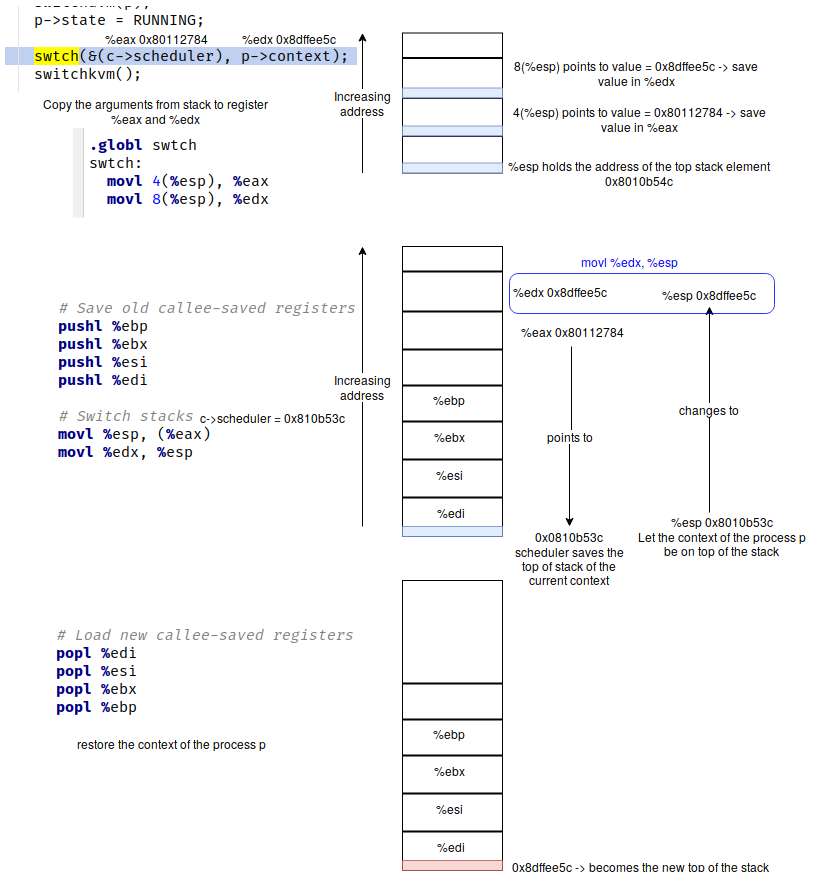
\includegraphics[width=\textwidth]{context_switch.png}
    \end{minipage}%
    \begin{minipage}[t]{0.5\textwidth}
        \vspace{-8cm} 
        \begin{itemize}[topsep=0pt, partopsep=0pt, itemsep=0pt, parsep=0pt]
            \item  When swtch function call is made, old kernel stack has return address (eip)
        and arguments to swtch (address of old context pointer, new context pointer)
        \item  Store address of old context pointer into eax
        \item  Store value of new context pointer into edx
        \item  Push callee save registers on kernel stack of old process
        \item Top of stack esp now points to complete context structure of old process
        \item  Update old context pointer (eax) to point to updated context
        \item  Switch stacks: Copy new context pointer from edx to esp
        \item  Pop registers from new context structure
        \item  Return from swtch in new process
        
        \end{itemize}
     
    \end{minipage}
    \caption{Assembly code in xv6 for \texttt{swtch()}}
    \label{fig:parallel}
\end{figure}

\subsubsection{\texttt{swtch()} for new processes}
Our way of working assumes the existence of a context structure of a process.
What if the process just started and has never run before (ie) a newly forked process?
The kernel stack of such new processes are setup\footnote{They are artificially setup with appropriate context sturcture and trap frame} in such a way that the EIP of function 
where the process starts from is saved in the context structure to mimic that the process
was switched out from where we want to resume in kernel mode(this location is just after the fork wherever our PC is pointing to). Apart from this the trap frame is copied
from the parent(\texttt{eax} or return value alone is changed for the \texttt{fork()}) so it has the proper \textit{register context} to resume in user mode just after wherever \texttt{fork()} call was made. Process resumes execution in kernel mode and it returns from trap to
user space(to the instruction right after the \texttt{fork()}).  


\textbf{allocproc:} This is the function that creates a new \textit{struct proc} for our newly forked process. It finds
an unused entry in the ptable and marks it as an embryo and changes it to runnable after the process completion is well "completed". It
also allocates a \textbf{PID} for this process along with new memory (ie) a kernel stack and also a stack pointer pointing to the bottom of this stack.
What else?
\begin{itemize}[topsep=0pt, partopsep=0pt, itemsep=0pt, parsep=0pt]
    \item Leave space for trapframe (copied from parent)
    \item after that pushes return address of “trapret”
    \item Push context structure, with \texttt{eip} pointing to
    function “forkret”. This is done since, when new process is scheduled, it begins
    execution at forkret, then returns to trapret, then returns from trap to userspace continuing to execute instructions after fork
    \item Thus we have hand-crafted kernel stack to make it look
    like process had a trap and context switch basically lying to the scheduler to make it like look like any process which was context switched in the past. So the OS scheduler can schedule it as it does
    any other process
\end{itemize}
\noindent\tbox{
    \begin{center}
    \textbf{\Huge Lecture 9}
    \end{center}
}

\subsection{OS Scheduling Policy}
Now that we have understood the mechanism of the OS scheduler let's see how the scheduler chooses which amongnst the 
ready processes it should run. An important point to note is that only when a process is in kernel mode for a trap a context switch happens. However not on every trap does the scheduler perform a context switch
The first classification among schedulers as we saw before are pre-emptive and non-premptive schedulers.
\begin{itemize}[topsep=0pt, partopsep=0pt, itemsep=0pt, parsep=0pt]
    \item \textbf{Pre-emptive:} Performs \textit{involuntary} context switches using timer interrupts\footnote{Refer \ref{section:Timer}}
    even if the process is in ready/runnable mode.
    \item \textbf{Non-preemptive:} Performs only voluntary context switches when a process gives up the control via a trap.
\end{itemize}

What are the goals of a scheduling policy?
\begin{itemize}[topsep=0pt, partopsep=0pt, itemsep=0pt, parsep=0pt]
    \item Maximise utilization: Efficient use of CPU hardware so that the throughput of the CPU is maximised
    \item Minimize the time it takes for a CPU to complete a process. It is also called as turnaround or completion time
    \item Minimize time it takes for the process to start running after it is ready to run which is called response time\footnote{Very important for processes that are highly interactive and constantly take input from users}
    \item Fairness is to be maintained (ie) all processes get a fair share of CPU (account for priorities also)
    \item We also want to minimize overhead. That is we don't want the scheduling itself to take too much processing power/time.
    We can't have unnecessarily large number of context switches (since it takes \(\sim \)1 microsecond to switch) or have too much time needed to take a decision even with larger number of processes to be scheduled
\end{itemize}


\subsection{Different scheduling policies}
\begin{enumerate}
    

    \item \textbf{FIFO(First in first out):}\\
    We put all our processes in a queue and then we run them one after another.
    Note that FIFO is non-preemptive (ie) a processes runs to termination or till it is blocked. In case of a blocked syscall, after it is done with handling
    a blocking syscall we add it to the end of the process as a new process with a new context. When it is added back it counts as a fresh CPU burst
    \footnote{A CPU burst is the time for which a process runs in a continuous stretch}

    \begin{table}[h]
        \centering
        \begin{tabular}{|c|c|c|c|}
        \hline
        \textbf{Process} & \textbf{CPU time needed} & \textbf{Arrives at end of} & \textbf{Execution time} \\
        \hline
        P1 & 5 & 0 & 1-5 \\
        \hline
        P2 & 3 & 1 & 6-8 \\
        \hline
        P3 & 2 & 3 & 9-10 \\
        \hline
        \end{tabular}
        \caption{FIFO}
        \label{tab:FIFO}
    \end{table}
    The disadvantages with FIFO is the convey effect (ie) processes which are shorter tend to get stuck behind much longer ones resulting in unnecessary increase in the turnaround time due to longer waiting time
   \item \textbf{Shortest Job First(SJF):} \\Asssuming that the scheduler has the knowledge on the CPU burst of all processes (time it runs for one continuous stretch). 
    Now we can pick the process with the shortest burst time first and run it and continue doing so. This can be done by maintaining all the processes
    in a heap ordered by burst time needed.
    \begin{table}[h]
        \centering
        \begin{tabular}{|c|c|c|c|}
        \hline
        \textbf{Process} & \textbf{CPU time needed} & \textbf{Arrives at end of} & \textbf{Execution time} \\
        \hline
        P1 & 5 & 0 & 1-5 \\
        \hline
        P2 & 3 & 1 & 8-10 \\
        \hline
        P3 & 2 & 3 & 6-7 \\
        \hline
        \end{tabular}
        \caption{Shortest Job First}
        \label{tab:SJF}
    \end{table}
    This can be proved to be the optimal solution when we assume all the processes arrive at the same time. However this is an unrealistic assumption.
    Also due to its non-preemptive nature short jobs can still get stuck behind longer ones (different arrival times). 

    \item \textbf{Shortest remaining time First(SRTF):} This is a preemptive version of \textbf{SJF}. A newly arrived process can preempt\footnote{terminate this process and make CPU context switch to itself} a running process, if 
    CPU burst of new process is shorter than remaining time of the running process. This avoids the problem of shorter process getting stuck behind longer ones if they don't arrive at the same time.
    
    \begin{table}[h]
        \centering
        \begin{tabular}{|c|c|c|c|}
        \hline
        \textbf{Process} & \textbf{CPU time needed} & \textbf{Arrives at end of} & \textbf{Execution time} \\
        \hline
        P1 & 5 & 0 & 1,\textit{preempted} then 7-10 \\
        \hline
        P2 & 3 & 1 & 2-4 \\
        \hline
        P3 & 2 & 3 & 5-6 \\
        \hline
        \end{tabular}
        \caption{Shortest Remaining Time First}
        \label{tab:SRTF}
    \end{table}
    However we are still assuming knowledge on the run times of processes before they arrive (unrealistic assumption).
\item \textbf{Round Robin(RR):}\\ This is the first practical policy we are seeing. We fix a time slice (called a quantum). The quantum is a multiple of the length of the timer interrupt.
So when the time interrupt happens the scheduler checks if the process has already run for the allocated time slice. If that is not the case, control is simply handed over back to the process. If not so, control is handed to another
runnable process by context switching into it. Thus the timer interrupt is used to enforce periodic scheduling. 
This policy is good for maintaining both response time and fairness, however it is not the most efficient for turnaround time. \texttt{xv6} uses this policy

What effect does time slice's length have?
\begin{itemize}[topsep=0pt, partopsep=0pt, itemsep=0pt, parsep=0pt]
    \item A small time slice makes it inefficient since too many context switch happen and the time spent to context switch isn't \href{https://english.stackexchange.com/a/138566}{amortized} properly
    \item If the time slice is too big there is no responsiveness as one process hoards the cpu for a longer time
\end{itemize}

\item \textbf{Weighted Fair Queueing(WFQ):} \\This is a modified version of Round Robin policy. We set weights to every process and give preferences according to it.
The weight setting is done by both user and the OS itself to different extents. The time slice is for a given a process is proportional to this weight. Real life schedulers may not be able to maintian the time slice enforcement accurately. Think about cases where the time interrupt
doesn't align with time share or a process is blocked before its slice. A practical modification to accomodate such things is to keep track of the run time of a process and switch in the process which has used the least fraction of its fair share. This compensates for deficiences/excess in the running time.
 
\item 
\textbf{CFS scheduler}:\\The Completely Fair Scheduler used in linux is a variant of WFQ. It uses red-black to keep track of who all runs and keeps track of who all have used up least amount of their fair share.
However it is impossible to be fully fair whilst being reasonable but this policy is close to optimal fairness.


\item \textbf{Multi-level feedback queue (MLFQ):} \\
This is another practical algorithm with realistic assumptions. We would prefer the property of the SJF which gives priority to smaller jobs. However we can't assume we know the running time before.
We also want to ensure that the response time is lesser as we see in Round robin. 

We have multiple queues corresponding to multiple priorities. Scheduling of processes happen first for higher priority queues and within a queue Round Robin is used for scheduling. If a process has used up more of its fair share of CPU we decay it's priority and push it down. When we 
add a process we add it to the high priority queue. This helps us have an idea on which process is running for a longer time and which ones haven't. We run and finish up shorted processes quickly (Like I/O) even without prior knowledge of CPU bursts. Periodically reset the priority level to make sure even longer
process gets some chance to run.
\end{enumerate}

\noindent\tbox{
    \begin{center}
    \textbf{\Huge Lecture 10}
    \end{center}
}

\subsection{Multicore Scheduling}
Scheduling decision is supposed to be made seperately for each core. Do we bind a process to a particular CPU core always or do we let a process,
run on any CPU core that is free? Making sure that the process runs on the same core as much as possible is better due to improved CPU cache performance.
However balancing is important, if the core is highly overloaded then we ensure a process runs on a different free core to not waste time. 

Overall however having
a single queue which assigns the ready process to the first free CPU out of all of the multiple CPU's present is more efficient than having
multiple queues for each CPU and choosing to put a process in one of these queues. This is due to the high cost and thus inability to switch queues once a process
is assigned a queue in the multiqueue case.


\section{Inter Process Communication}
Why do we need IPC\footnote{Interprocess Communication}? In real life systems it is not ideal or feasible to maintain all of the functionality in just a single
process. Rather we 
modularise code (which can be in different languages, frameworks and written by different teams of people) and need some method for them to work along with each other.

Processes in a system needn't share memory with each other by default. However they still need the ability to communicate. This is done via
IPC mechanisms, which are available via the OS whcih provides several syscalls enabling the exchange of information between processes. The communication can also
be done by two processes agreeing to share a particular portion of the memory image to enable communication. Communication can also be done by having a particular
memory area (buffer) specifically meant for communication. It is important to note that it is an extremely dumb idea to just let two processes have access to the entire 
memory images of each other since this destroys the ability to maintain isolation of processes.   


\subsection{Sockets:}
Sockets are an abstraction to enable communication between processes. Each process opens its own socket and two sockets of two processes can be connected.
The process to open the socket first is the \textit{server} and the process which connects its socket to the server is the \textit{client}. A socket is a way of 
bidirectional communication, thus a process can write into its socket which can be read by other processes and vice versa. Processes communicating using socktes can be 
in the same machine or on different machines. While communicating on the same machine the buffer\footnote{intermediate storage which stores message to be sent} is present in OS memory. For communicating across machines messages are sent on the network.
\textit{Unix Domain sockets} are used to communicate between processes on the same machine. \textit{Internet sockets} are used to communicate between
processes on different machines. 


The client needs some information about the process whose socket it wants to connect to (server). Thus every socket needs a unique number
to identify itself. This \texttt{ID} for a Internet socket is the IP address and port number. Local sockets are identified a unique \textit{pathname} identifying it in the local machine. Note that the local
socket isn't exactly a file but it has a pathname that only serves the purpose of identying it uniquely.
The server needs to publicise its identifier (IP or pathname) for the client process to know where to connect to.


\textit{Connection-based sockets} are those when a client and server are explicitly connected to each other. After this connection they can only talk to each other. So there is no need to explicitly mention which socket we want to communicate to.
\textit{Connection-less sockets} are those who can communicate with multiple processes at the same time. Thus we need to mention the address of the socket we want to communicate with. 


\subsubsection{\texttt{socket()} syscall}
The \texttt{socket()} syscall is used to create a socket. It takes the type of socket as an argument and returns the file descriptor of the socket to the process. This file descriptor 
is used for all operations on the socket by this process. A socket can optionally bind to the address (pathname or IP address/port number) using \texttt{bind()} system call. 
Server socket binding means that the socket is given a global address which can be used by other processes to communicate to this socket. Note that binding is compulsory for server sockets who need to 
publicise this binding address to enable clients to talk to them. The \texttt{close()} system call closes a socket.


How do processes use \textbf{sockets} to communicate?
\begin{itemize}
    \item \textbf{sendto():} is used to send a message from one socket to another connection-less socket. It takes its own socket's file descriptor, the message to be sent, the other socket's address as arguments
    \item \textbf{recvfrom():} is used to recieve a message from a socket. It takes the its socket's file descriptor, a message buffer to copy the message into and a sockets address structure into which the recieving socket's
    global address is filled. Now this process can use the address it just obtained to communicate back to the process which sent it a message. 
\end{itemize}

\noindent\tbox{
    \begin{center}
    \textbf{\Huge Lecture 11}
    \end{center}
}
\subsubsection*{Connecting sockets}
Connection-oriented sockets need to be explicitly connected for transfer of messages.
After a server binds to a well-known address\footnote{gets assigned a proper global address}, it uses the \texttt{listen()} syscall to listen
for "requests to connect" from clients who want to connect to server. Clients use the \texttt{connect()} to send a request to connect to the server. The server
uses \texttt{accept()} syscall to accept a request from the client to establish a connection. Once an \texttt{accept()} syscall is sucessfull then a connection
is established between the client and server. 


The \texttt{accept()} syscall takes the file descriptor of a socket as an argument. This socket's address is what clients use to send a "request to connect".
Once the \texttt{accept()} syscall is succesful it returns a \textbf{new file descriptor} to a socket which is connected to the client. 

Hence it is important to note that there is a \textit{listening socket} corresponding to whose address requests are send to connect and there are (possibly multiple)
\textit{connected sockets} explicitly connected to a client socket to enable communication between two unique processes. 
The \texttt{accept()} syscall will block the server till is recieves a request to connect from a client. Similarly, the \texttt{connect()} syscall blocks the client till the server accepts the requests.

After a client connects to a server, the \textit{pair of sockets} are used to exchange data. Again let's reassert that the \textit{connected socket} is the one which is used to transfer messages not the \textit{listen socket}.
Syscall \texttt{send/write} to send a message which only goes to the connected socket.
Similarly syscall \texttt{recv()/read()} is used to recieve a message on connected socket. 
The arguments given to send/recv are the socket fd, message buffer, buffer length and (optional) flags.
The return value is number of bytes read/written or error number.
We need not specify socket address on every message, as they connected already and only communicate with each other using that particular socket.

In any kind of real system multiple connected and connection-less sockets connect multiple processes in several ways forming a complex network of processes all working with one another to achieve some task. 

\subsection{Message queues}
Message queues are another method used for exchanging messages between processes. We open a connection to a message queue identified by a "key", and get a file descriptor to it. The sender can open a connection to
the message queue and send a message. The reciever opens a connection to the message queue and recieves the message later on. The message queue acts as a buffer till the message is retrieved by a reciever.


There are three main syscalls associated with a message queue:
\begin{itemize}[topsep=0pt, partopsep=0pt, itemsep=0pt, parsep=0pt]
    \item \texttt{msgget()}: syscall to get the id of a message queue. The parameters it takes are the key of the message queue . It returns the msg\_queue identifier on success and -1 on failure.
    \item \texttt{msgsnd()}: The parameters it takes are the msg\_queue identifier and the message to be sent and its size. It returns 0 on success and -1 on failure. 
    \item \texttt{msgrcv()}: The parameters it takes are the msg\_queue identifier, size of the message and the buffer to write the message into. It returns the number of bytes recieved on success and -1 on failure.
\end{itemize}
There can be several different message queues all with their own unique "keys". Also note that multiple processes can use the same message queue if they all have access to its key. Thus we need to be careful about which process's message is being recieved when \texttt{msgrcv()} is used.

\subsection{Pipes}
A pipe is a unidirectional FIFO channel into which writing is done on one end and reading from another end. The syscall \texttt{pipe()} is used to create a unidirectional pipe. It returns two file descriptors for 
the end points (one for write, other for read). A pointer to a \texttt{struct} of a pair of numbers are passed as a parameters of the pipe. Once a pipe is succesful this \texttt{struct} has both file descriptors. Why do we have access to both descriptors? This is because Pipes
are frequently used for communication between a parent and a child. The data written into a pipe is stored in the buffer of the pipe channel until they are read. Obviously, bi-directional communication between two processes needs two pipes. 


\textbf{Anonymous pipes} are only available to communicate between process and its children. The pipe file descriptor is available to both the parent and the child.

\textbf{Named pipes} are used by two unrelated processes to talk to each other. The pipe is opened with a pathname which is accessible across processes. One of the processes
has access to the read end of a pipe, while the other other process opens the write end. 


\textbf{Buffer Mechanism:}  
When we want to send a message the general mechanism stays the same across all these sycalls. We write the message into a temporary space called the buffer. This buffer is usually some memory location
inside OS not directly accessible by the user.
In all of these system calls the buffer maintains the messages in a FIFO order. When the buffer is read the message which was in it and was read is cleared. Sender 
usually can't be blocked by \texttt{send()} syscall unless the temporary buffer is full. Similarly reciever can be blocked if temporary buffer is empty. We can also customize the sycalls to not block the process
but return some error code for us to handle to error manually.

\subsection{Shared memory}
Processes in a system do not share any memory unless mentioned otherwise. Child process \textit{copies} the memory of the parent but doesn't share the memory image.
Shared memory means that the same memory image appears in multiple processes. Each memory \textit{segment} shared is identified by a unique key. A process can request to map/attach this shared 
memory segment into its own memory image using this identifier key. 

Sharing of memory is a risky and volatile task. The processes thus need extra mechanisms to know for example, if the memory has been modified. This enables them to coordinate with one another


\noindent\tbox{
    \begin{center}
    \textbf{\Huge Lecture 12}
    \end{center}
}
\section{Memory Management}
\subsection*{Abstraction of Address space}
Every process assumes it has access to a large space of memory from address 0 to a max value. The maximum value depends on the available number of bits for the memory space.
The virtual address sapce contains all the code/data that a process can access. Addresses in CPU registers point to these virtual addresses.




However this is not how memory is actually stored. The OS maintains this illusion of virtualized address spaces by having a map from every virtual address to a physical address. When the CPU accesses memory 
using an address (virtual address) the Memory Management Unit (MMU) converts it to a real address and gives back the data at the physical memory corresponding to the virtual address. OS allocates physical memory to a process, it has the translation information
provides it to MMU.

Why do we need the MMU? Why not the OS? This is primarily since we don't want to trap into the kernel for every memory access. The OS does the background work
of allocating memory for processes and maintaing the virtual address $\rightarrow$ physical address mapping and simply passes on the information to the MMU.
The MMU deals with translation of virtual memory to real memory. During Bootup the OS starts on the MMU and starts giving it translation information.

\begin{figure}
    \begin{center}
        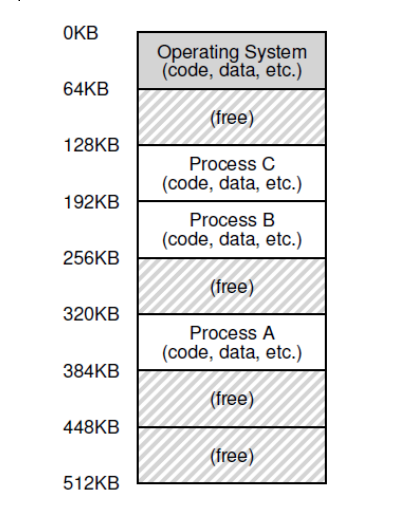
\includegraphics[width = 6cm]{memory_allocation.png}
        \label{figure:memory_alloc}
        \caption{Memory allocation for three processes}
    \end{center}
\end{figure}


\subsubsection*{Why virtual address?}
The real view of memory is messy and it is not easy to manage manually. In earlier systems there was only one process and its own code. Nowadays we have multiple
parallely running processes which all do time\-sharing on the same CPU. Memory is also allocated in a non-contiguos manner, but we still want to maintain the illusion of memory being continuosly allocated. 
Thus virtualization has become a neccesity in modern systems. The CPU \textbf{only} uses the virtual addresses to perform any action.\footnote{For example addresses of a pointer obtained from \texttt{malloc()} is the virtual address}

\subsection{Base and bound}
This is the simplest form of memory management. It is not used in modern systems but we will understand it to get some insights. The memory image
from [0,N] is placed at memory address base B. That is every virtual address X is stored at physical address B + X. There is also a bound associated with this base which tells us 
the maximal address for the memory allocated in this memory image.



Simple example: Let's take a small porgram as given hello

\begin{lstlisting}
    void func(){
        int x = 300;
        x = x + 3;
    }
\end{lstlisting}
This code compiles to give instructions. 

Suppose the OS places the entire memory image in one chunk starting at physical address 32kb, then the OS indicates base and bound to MMU. 
MMU performs this translation from Virtual adress to physical address. But what if some garbage address/ out of bound address is given? Then the
MMU raises a trap to call the OS to handle this situation. This is another type of hardware level trap (program fault). In this case int n is inserted into the 
stream of instructions run by the CPU. 

\subsection{OS vs MMU}
The OS is the one who allocates the memory and builds the translation information of a process. However the MMU
is the one who translates virtual address to a physical address. Note that once the user starts running the OS is out of the picture unless there is a trap.

When a context switch happens the OS changes the translation information in the MMU to enable it to perform translating addresses corresponding to this new process \footnote{same virtual address means different physical address in different processes}. 
As told before when the CPU has an instruction which wants to access memory the MMU translates it to a physical address which can be used to access the data.

\subsection{Segmenation}
It is an upgradation of base and bound. The program is split into several segments (Code, data, stack) and each of them is placed at a different memory location (base).
Each of these bases also have a bound associated with them. When the address exceeds the bound of a segment we obtain a \textit{segmenation fault}\footnote{\href{https://www.youtube.com/watch?v=NAEppFUWLfc}{\textit{sigh}}}
. Thus when we context switch into a process the OS updates the MMU with all the necessary bases and bounds.
Each virtual address is hence a segment identifier bit sequence concatenated with an offset for that particular byte.

But this is still inefficient due to the variable sizes of these segments. This also results in \textit{fragmentation} where there is some unusable space between two segments. 

\subsection{Paging}
Paging is the mostly widely used system of memory Management today. We divide our virtual address space into fixed size pages. Each one of these pages is assigned a free \textbf{physical frame}\footnote{Just the physical memory associated with a single page}.
The memory allocation for each page is done at a fixed size (eg. 4kb). Since the pages are tightly packed we have no wasteage of size between pages (ie) no \textit{external fragmentation}. However inside the pages we could have some wasteage of space (ie) \textit{internal fragmentation}.

What is the optimal page size? Why 4kb?
\begin{itemize}[topsep=0pt, partopsep=0pt, itemsep=0pt, parsep=0pt]
    \item \textit{Large page size} \(\rightarrow\) larger amount of wastage inside individual pages.
    \item \textit{Small page size} \(\rightarrow\) OS has to keep track of huge number of pages which creates a large overhead.\footnote{Large processing power is needed to maintain page table}
\end{itemize}
\noindent\tbox{
    \begin{center}
    \textbf{\Huge Lecture 13}
    \end{center}
}
\subsection{Page table}
\subsubsection*{What is a page table?}
The page table is a per process structure (ie) each process has its own page table. This table helps to translate
virtual addresses to real ones. It stores frame numbers for all the pages used by the process in an array format. 
Table[i] gives the physical frame number of the ith virtual page of the process. Thus the ith entry of the page table corresponds to the physical address of the starting byte of the ith page. The page table is stored in a part of a OS memory (stored in PCB). The MMU has 
access to the page tables of current processes and it uses it for translation. 


Given page table of a process, how is physical address obtained from virtual address?

When you have the virtual address you can find which page your data is in. This can be done by (Virtual Address / Page size) and the offset is (Virtual Address \% Page size).
That is the most significant digits give the page number and the least significant ones give the offset. 

\begin{figure}
    \begin{center}
        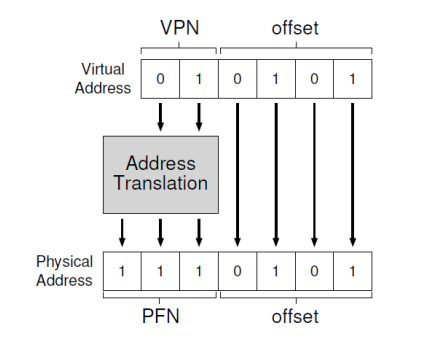
\includegraphics[width = 6cm]{address_translation.png}
        \label{figure:address_translation}
        \caption{Visual representation of address translation}
    \end{center}
\end{figure}


Hence the most significant digits give the Virtual Page Number (VPN) and least significant bytes give the offset. The VPN and the page
table can be used to get the Physical Frame Number. Note that Page\_Table\_array[VPN] = PFN\footnote{Physical Frame Number}. Obviously the offset to get the byte
we want is same in both the Physical frame and the virtual page.

\subsubsection*{Translation Lookaside Buffer(TLB)}
An important point to note with paging is that one memory access has become two accesses now. One access to the page table and the one to the actual byte we want. This results in a significant
slow down since memory accesses are very slow. This is the overhead associated with paging

To reduce this overhead the MMU caches the most recent translations in translation lookaside buffer(TLB)\footnote{It is a fully associated cache}.
TLB caches only the \textbf{page table entries} \footnote{the physical data in 32/64 bit addresses are cached by the actual cpu cache}. If we have
a hit, we fetch the memory contents of the given address in one access since we already have the page table entry in the cache. If there is a miss we get the memory from RAM and place it in TLB for future accesses after 
which we use the translated address and then again use this page table entry to translate the virtual address and get the memory we wanted.

Interestingly, during a context switch the TLB is flushed. This is due to the fact that the MMU needs to translate the Page table for every processes in a different
way (different page table entries).


Thus the TLB is very important and \textit{needs} to have a high hit rate. It works parallely with the CPU cache to further optimize memory accesses.  

\end{document}